\documentclass[twoside]{book}

% Packages required by doxygen
\usepackage{fixltx2e}
\usepackage{calc}
\usepackage{doxygen}
\usepackage[export]{adjustbox} % also loads graphicx
\usepackage{graphicx}
\usepackage[utf8]{inputenc}
\usepackage{makeidx}
\usepackage{multicol}
\usepackage{multirow}
\PassOptionsToPackage{warn}{textcomp}
\usepackage{textcomp}
\usepackage[nointegrals]{wasysym}
\usepackage[table]{xcolor}

% Font selection
\usepackage[T1]{fontenc}
\usepackage[scaled=.90]{helvet}
\usepackage{courier}
\usepackage{amssymb}
\usepackage{sectsty}
\renewcommand{\familydefault}{\sfdefault}
\allsectionsfont{%
  \fontseries{bc}\selectfont%
  \color{darkgray}%
}
\renewcommand{\DoxyLabelFont}{%
  \fontseries{bc}\selectfont%
  \color{darkgray}%
}
\newcommand{\+}{\discretionary{\mbox{\scriptsize$\hookleftarrow$}}{}{}}

% Page & text layout
\usepackage{geometry}
\geometry{%
  a4paper,%
  top=2.5cm,%
  bottom=2.5cm,%
  left=2.5cm,%
  right=2.5cm%
}
\tolerance=750
\hfuzz=15pt
\hbadness=750
\setlength{\emergencystretch}{15pt}
\setlength{\parindent}{0cm}
\setlength{\parskip}{3ex plus 2ex minus 2ex}
\makeatletter
\renewcommand{\paragraph}{%
  \@startsection{paragraph}{4}{0ex}{-1.0ex}{1.0ex}{%
    \normalfont\normalsize\bfseries\SS@parafont%
  }%
}
\renewcommand{\subparagraph}{%
  \@startsection{subparagraph}{5}{0ex}{-1.0ex}{1.0ex}{%
    \normalfont\normalsize\bfseries\SS@subparafont%
  }%
}
\makeatother

% Headers & footers
\usepackage{fancyhdr}
\pagestyle{fancyplain}
\fancyhead[LE]{\fancyplain{}{\bfseries\thepage}}
\fancyhead[CE]{\fancyplain{}{}}
\fancyhead[RE]{\fancyplain{}{\bfseries\leftmark}}
\fancyhead[LO]{\fancyplain{}{\bfseries\rightmark}}
\fancyhead[CO]{\fancyplain{}{}}
\fancyhead[RO]{\fancyplain{}{\bfseries\thepage}}
\fancyfoot[LE]{\fancyplain{}{}}
\fancyfoot[CE]{\fancyplain{}{}}
\fancyfoot[RE]{\fancyplain{}{\bfseries\scriptsize Generated by Doxygen }}
\fancyfoot[LO]{\fancyplain{}{\bfseries\scriptsize Generated by Doxygen }}
\fancyfoot[CO]{\fancyplain{}{}}
\fancyfoot[RO]{\fancyplain{}{}}
\renewcommand{\footrulewidth}{0.4pt}
\renewcommand{\chaptermark}[1]{%
  \markboth{#1}{}%
}
\renewcommand{\sectionmark}[1]{%
  \markright{\thesection\ #1}%
}

% Indices & bibliography
\usepackage{natbib}
\usepackage[titles]{tocloft}
\setcounter{tocdepth}{3}
\setcounter{secnumdepth}{5}
\makeindex

% Hyperlinks (required, but should be loaded last)
\usepackage{ifpdf}
\ifpdf
  \usepackage[pdftex,pagebackref=true]{hyperref}
\else
  \usepackage[ps2pdf,pagebackref=true]{hyperref}
\fi
\hypersetup{%
  colorlinks=true,%
  linkcolor=blue,%
  citecolor=blue,%
  unicode%
}

% Custom commands
\newcommand{\clearemptydoublepage}{%
  \newpage{\pagestyle{empty}\cleardoublepage}%
}

\usepackage{caption}
\captionsetup{labelsep=space,justification=centering,font={bf},singlelinecheck=off,skip=4pt,position=top}

%===== C O N T E N T S =====

\begin{document}

% Titlepage & ToC
\hypersetup{pageanchor=false,
             bookmarksnumbered=true,
             pdfencoding=unicode
            }
\pagenumbering{alph}
\begin{titlepage}
\vspace*{7cm}
\begin{center}%
{\Large rwa2-\/ngo }\\
\vspace*{1cm}
{\large Generated by Doxygen 1.8.13}\\
\end{center}
\end{titlepage}
\clearemptydoublepage
\pagenumbering{roman}
\tableofcontents
\clearemptydoublepage
\pagenumbering{arabic}
\hypersetup{pageanchor=true}

%--- Begin generated contents ---
\chapter{File Index}
\section{File List}
Here is a list of all files with brief descriptions\+:\begin{DoxyCompactList}
\item\contentsline{section}{\hyperlink{main_01__backup_8cpp}{main \+\_\+backup.\+cpp} }{\pageref{main_01__backup_8cpp}}{}
\item\contentsline{section}{\hyperlink{main_8cpp}{main.\+cpp} }{\pageref{main_8cpp}}{}
\end{DoxyCompactList}

\chapter{File Documentation}
\hypertarget{main_01__backup_8cpp}{}\section{main \+\_\+backup.\+cpp File Reference}
\label{main_01__backup_8cpp}\index{main \+\_\+backup.\+cpp@{main \+\_\+backup.\+cpp}}
{\ttfamily \#include $<$iostream$>$}\newline
Include dependency graph for main \+\_\+backup.\+cpp\+:\nopagebreak
\begin{figure}[H]
\begin{center}
\leavevmode
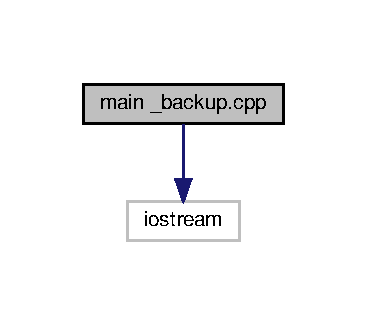
\includegraphics[width=176pt]{main_01__backup_8cpp__incl}
\end{center}
\end{figure}
\subsection*{Functions}
\begin{DoxyCompactItemize}
\item 
bool \hyperlink{main_01__backup_8cpp_abfa7bcedc52eb1d5a7962f1b48106a8f}{Find\+Path} (int x, int y)
\item 
int \hyperlink{main_01__backup_8cpp_ae66f6b31b5ad750f1fe042a706a4e3d4}{main} ()
\end{DoxyCompactItemize}


\subsection{Function Documentation}
\mbox{\Hypertarget{main_01__backup_8cpp_abfa7bcedc52eb1d5a7962f1b48106a8f}\label{main_01__backup_8cpp_abfa7bcedc52eb1d5a7962f1b48106a8f}} 
\index{main \+\_\+backup.\+cpp@{main \+\_\+backup.\+cpp}!Find\+Path@{Find\+Path}}
\index{Find\+Path@{Find\+Path}!main \+\_\+backup.\+cpp@{main \+\_\+backup.\+cpp}}
\subsubsection{\texorpdfstring{Find\+Path()}{FindPath()}}
{\footnotesize\ttfamily bool Find\+Path (\begin{DoxyParamCaption}\item[{int}]{x,  }\item[{int}]{y }\end{DoxyParamCaption})}

\mbox{\Hypertarget{main_01__backup_8cpp_ae66f6b31b5ad750f1fe042a706a4e3d4}\label{main_01__backup_8cpp_ae66f6b31b5ad750f1fe042a706a4e3d4}} 
\index{main \+\_\+backup.\+cpp@{main \+\_\+backup.\+cpp}!main@{main}}
\index{main@{main}!main \+\_\+backup.\+cpp@{main \+\_\+backup.\+cpp}}
\subsubsection{\texorpdfstring{main()}{main()}}
{\footnotesize\ttfamily int main (\begin{DoxyParamCaption}{ }\end{DoxyParamCaption})}


\hypertarget{main_8cpp}{}\section{main.\+cpp File Reference}
\label{main_8cpp}\index{main.\+cpp@{main.\+cpp}}
{\ttfamily \#include $<$iostream$>$}\newline
Include dependency graph for main.\+cpp\+:\nopagebreak
\begin{figure}[H]
\begin{center}
\leavevmode
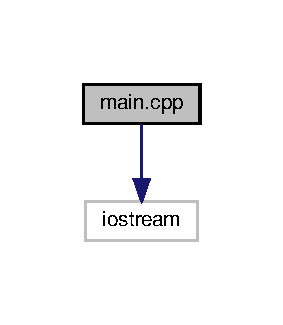
\includegraphics[width=136pt]{main_8cpp__incl}
\end{center}
\end{figure}
\subsection*{Macros}
\begin{DoxyCompactItemize}
\item 
\#define \hyperlink{main_8cpp_a3cfd3aa62338d12609f6d65bce97e9cd}{R\+O\+WS}~6
\begin{DoxyCompactList}\small\item\em Number of Rows for the Maze. \end{DoxyCompactList}\item 
\#define \hyperlink{main_8cpp_ab59ad2ee1a48b83c2eef1f019ed8cc48}{C\+O\+LS}~8
\begin{DoxyCompactList}\small\item\em Number of Columns for the Maze. \end{DoxyCompactList}\end{DoxyCompactItemize}
\subsection*{Functions}
\begin{DoxyCompactItemize}
\item 
bool \hyperlink{main_8cpp_acfa4bb7c74cebff4cd34982630e27e5a}{Check\+Wall} (char maze\mbox{[}6\mbox{]}\mbox{[}8\mbox{]}, int \&x, int \&y)
\item 
bool \hyperlink{main_8cpp_a15ab7ba904c0f46588d62b302075a8c3}{Check\+Outside} (int \&x, int \&y)
\item 
bool \hyperlink{main_8cpp_aefd146022809df49fb9ba712ecb00ffe}{Back\+Track} (char maze\mbox{[}6\mbox{]}\mbox{[}8\mbox{]}, int \&x, int \&y)
\item 
void \hyperlink{main_8cpp_a41b5491830aa7fa26ded753af127966f}{display\+\_\+maze} (char maze\mbox{[}6\mbox{]}\mbox{[}8\mbox{]})
\item 
bool \hyperlink{main_8cpp_acafe6eccc9f6c953bc9b609f732b2273}{Find\+Path} (char maze\mbox{[}6\mbox{]}\mbox{[}8\mbox{]}, int x, int y)
\item 
int \hyperlink{main_8cpp_ae66f6b31b5ad750f1fe042a706a4e3d4}{main} ()
\end{DoxyCompactItemize}


\subsection{Macro Definition Documentation}
\mbox{\Hypertarget{main_8cpp_ab59ad2ee1a48b83c2eef1f019ed8cc48}\label{main_8cpp_ab59ad2ee1a48b83c2eef1f019ed8cc48}} 
\index{main.\+cpp@{main.\+cpp}!C\+O\+LS@{C\+O\+LS}}
\index{C\+O\+LS@{C\+O\+LS}!main.\+cpp@{main.\+cpp}}
\subsubsection{\texorpdfstring{C\+O\+LS}{COLS}}
{\footnotesize\ttfamily \#define C\+O\+LS~8}



Number of Columns for the Maze. 

\mbox{\Hypertarget{main_8cpp_a3cfd3aa62338d12609f6d65bce97e9cd}\label{main_8cpp_a3cfd3aa62338d12609f6d65bce97e9cd}} 
\index{main.\+cpp@{main.\+cpp}!R\+O\+WS@{R\+O\+WS}}
\index{R\+O\+WS@{R\+O\+WS}!main.\+cpp@{main.\+cpp}}
\subsubsection{\texorpdfstring{R\+O\+WS}{ROWS}}
{\footnotesize\ttfamily \#define R\+O\+WS~6}



Number of Rows for the Maze. 



\subsection{Function Documentation}
\mbox{\Hypertarget{main_8cpp_aefd146022809df49fb9ba712ecb00ffe}\label{main_8cpp_aefd146022809df49fb9ba712ecb00ffe}} 
\index{main.\+cpp@{main.\+cpp}!Back\+Track@{Back\+Track}}
\index{Back\+Track@{Back\+Track}!main.\+cpp@{main.\+cpp}}
\subsubsection{\texorpdfstring{Back\+Track()}{BackTrack()}}
{\footnotesize\ttfamily bool Back\+Track (\begin{DoxyParamCaption}\item[{char}]{maze\mbox{[}6\mbox{]}\mbox{[}8\mbox{]},  }\item[{int \&}]{x,  }\item[{int \&}]{y }\end{DoxyParamCaption})}

Function to backtrack if the coordinate has been visited and there is no path found 
\begin{DoxyParams}{Parameters}
{\em maze} & the 2D array of character for the maze \\
\hline
{\em x} & integer of the x coordinate \\
\hline
{\em y} & integer of the y coordinate \\
\hline
\end{DoxyParams}
\begin{DoxyReturn}{Returns}

\end{DoxyReturn}
\mbox{\Hypertarget{main_8cpp_a15ab7ba904c0f46588d62b302075a8c3}\label{main_8cpp_a15ab7ba904c0f46588d62b302075a8c3}} 
\index{main.\+cpp@{main.\+cpp}!Check\+Outside@{Check\+Outside}}
\index{Check\+Outside@{Check\+Outside}!main.\+cpp@{main.\+cpp}}
\subsubsection{\texorpdfstring{Check\+Outside()}{CheckOutside()}}
{\footnotesize\ttfamily bool Check\+Outside (\begin{DoxyParamCaption}\item[{int \&}]{x,  }\item[{int \&}]{y }\end{DoxyParamCaption})}

Check\+Outside Function\+: Function to check if the desired direction is outside of the maze 
\begin{DoxyParams}{Parameters}
{\em maze} & the 2D array of character for the maze \\
\hline
{\em x} & integer of the x coordinate \\
\hline
{\em y} & integer of the y coordinate \\
\hline
\end{DoxyParams}
\begin{DoxyReturn}{Returns}

\end{DoxyReturn}
\mbox{\Hypertarget{main_8cpp_acfa4bb7c74cebff4cd34982630e27e5a}\label{main_8cpp_acfa4bb7c74cebff4cd34982630e27e5a}} 
\index{main.\+cpp@{main.\+cpp}!Check\+Wall@{Check\+Wall}}
\index{Check\+Wall@{Check\+Wall}!main.\+cpp@{main.\+cpp}}
\subsubsection{\texorpdfstring{Check\+Wall()}{CheckWall()}}
{\footnotesize\ttfamily bool Check\+Wall (\begin{DoxyParamCaption}\item[{char}]{maze\mbox{[}6\mbox{]}\mbox{[}8\mbox{]},  }\item[{int \&}]{x,  }\item[{int \&}]{y }\end{DoxyParamCaption})}

Check\+Wall Function\+: Function to check if there is a wall in the desired direction 
\begin{DoxyParams}{Parameters}
{\em maze} & the 2D array of character for the maze \\
\hline
{\em x} & integer of the x coordinate \\
\hline
{\em y} & integer of the y coordinate \\
\hline
\end{DoxyParams}
\begin{DoxyReturn}{Returns}

\end{DoxyReturn}
\mbox{\Hypertarget{main_8cpp_a41b5491830aa7fa26ded753af127966f}\label{main_8cpp_a41b5491830aa7fa26ded753af127966f}} 
\index{main.\+cpp@{main.\+cpp}!display\+\_\+maze@{display\+\_\+maze}}
\index{display\+\_\+maze@{display\+\_\+maze}!main.\+cpp@{main.\+cpp}}
\subsubsection{\texorpdfstring{display\+\_\+maze()}{display\_maze()}}
{\footnotesize\ttfamily void display\+\_\+maze (\begin{DoxyParamCaption}\item[{char}]{maze\mbox{[}6\mbox{]}\mbox{[}8\mbox{]} }\end{DoxyParamCaption})}

Function to display the maze 
\begin{DoxyParams}{Parameters}
{\em maze} & the 2d array of characters for the maze \\
\hline
\end{DoxyParams}
\mbox{\Hypertarget{main_8cpp_acafe6eccc9f6c953bc9b609f732b2273}\label{main_8cpp_acafe6eccc9f6c953bc9b609f732b2273}} 
\index{main.\+cpp@{main.\+cpp}!Find\+Path@{Find\+Path}}
\index{Find\+Path@{Find\+Path}!main.\+cpp@{main.\+cpp}}
\subsubsection{\texorpdfstring{Find\+Path()}{FindPath()}}
{\footnotesize\ttfamily bool Find\+Path (\begin{DoxyParamCaption}\item[{char}]{maze\mbox{[}6\mbox{]}\mbox{[}8\mbox{]},  }\item[{int}]{x,  }\item[{int}]{y }\end{DoxyParamCaption})}

Find\+Path Function is a recursive function to iterate through the maze by checking North, East, South, and West. It checks if there is a wall at the position or if its outside of the maze, then proceeds by placing a + sign at the position and updates. 
\begin{DoxyParams}{Parameters}
{\em maze} & the 2D array of character for the maze \\
\hline
{\em x} & integer of the x coordinate \\
\hline
{\em y} & integer of the y coordinate \\
\hline
\end{DoxyParams}
\begin{DoxyReturn}{Returns}

\end{DoxyReturn}
If the x, y is at the goal position

If the coordinates is not at the goal position

Declare outside variable

Declare wall variable

Declare backtrack variable

If x, y is outside of the maze or is a wall

Mark path

Checking North

Checking East

Checking South

Checking West

Backtrack by setting the coordinate back to . \mbox{\Hypertarget{main_8cpp_ae66f6b31b5ad750f1fe042a706a4e3d4}\label{main_8cpp_ae66f6b31b5ad750f1fe042a706a4e3d4}} 
\index{main.\+cpp@{main.\+cpp}!main@{main}}
\index{main@{main}!main.\+cpp@{main.\+cpp}}
\subsubsection{\texorpdfstring{main()}{main()}}
{\footnotesize\ttfamily int main (\begin{DoxyParamCaption}{ }\end{DoxyParamCaption})}

Maze array is reversed to print it out with respect to the coordinate system

Initialize the variables for the starting position

Initialize temporary variables s\+\_\+x and s\+\_\+y to save the new input

User Input

While Loop to determine if start and goal position are inside of the maze and not a wall

This if loop checks if the desired starting position is outside of the maze.

set the s array to coordinates x, y

Initialize temporary variables g\+\_\+x and g\+\_\+y to save the new input

This if loop checks if the desired goal position is outside of the maze.

set the g array to coordinates x, y 
%--- End generated contents ---

% Index
\backmatter
\newpage
\phantomsection
\clearemptydoublepage
\addcontentsline{toc}{chapter}{Index}
\printindex

\end{document}
